
%%%%%%%%%%%%%%%%%%%%%%%%%%%%%%%%%%%%%%%%%%%%%%%%%%%%%%%%%%%%%%%%%%%%%%%%%%%%%%%%
%
% Gadget2
%
%%%%%%%%%%%%%%%%%%%%%%%%%%%%%%%%%%%%%%%%%%%%%%%%%%%%%%%%%%%%%%%%%%%%%%%%%%%%%%%%

\section{Simulations with \gadgettwo}
\label{sec:gadget}

%%%%%%%%%%%%%%%%%%%%%%%%%%%%%%%%%%%%%%%%%%%%%%%%%%%%%%%%%%%%%%%%%%%%%%%%%%%%%%%%


We use the massively parallel TreeSPH \citep{1989ApJS...70..419H} cosmological \nbody\ simulation code \gadgettwo\ \citep{2001NewA....6...79S, 2005MNRAS.364.1105S} for the dark matter simulations presented in this work.  In this section, we give an overview of the fundamentals of the \gadgettwo\ code, followed by details of our particular simulations.




%~~~~~~~~~~~~~~~~~~~~~~~~~~~~~~~~~~~~~~~~~~~~~~~~~~~~~~~~~~~~~~~~~~~~~~~~~~~~~~~
\subsection{\gadgettwo}
\label{subsec:gadget--gadget}
%~~~~~~~~~~~~~~~~~~~~~~~~~~~~~~~~~~~~~~~~~~~~~~~~~~~~~~~~~~~~~~~~~~~~~~~~~~~~~~~


\gadgettwo\ is a massively parallel cosmological \nbody\ simulation code which calculates gravitational forces via a hierarchical multipole expansion and ideal gas parameters via smoothed particle hydrodynamics \citep[SPH; ][]{1977MNRAS.181..375G}.  This section will discuss the gravitational algorithms used to compute forces and the time integration method used to advance the simulation.  As our simulations are collisionless only, we do not discuss the details of the implementation of gas dynamics in \gadgettwo.



%:::::::::::::::::::::::::::::::::::::::::::::::::::::::::::::::::::::::::::::::
\subsubsection{Gravitational Algorithms}
\label{subsubsec:gadget--gadget--gravitational_algorithms}
%:::::::::::::::::::::::::::::::::::::::::::::::::::::::::::::::::::::::::::::::


Force computation suffers from a numerical singularity as the separation between two particles approaches zero, as discussed in Section~\ref{subsec:computational_theory--nbody_simulations}.  A modification of the force law is therefore required at small separation scales.  Force softening is accomplished in \gadgettwo\ using a spline kernel \citep{1985A&A...149..135M} $W(|x|, h = 2.8 \epsilon)$, where
\begin{equation} \label{eq:gadget--gadget--spline_kernel}
	W(r,h) = \frac{8}{\pi h^{3}}
	\begin{cases}
		1 - 6 \left( \frac{r}{h} \right)^{2} + 6 \left( \frac{r}{h} \right)^{3}, & 0 \leq \frac{r}{h} \leq \frac{1}{2} \\
		2 \left( 1 - \frac{r}{h} \right)^{3},                                    & \frac{1}{2} < \frac{r}{h} \leq 1, \\
		0,                                                                       & \frac{r}{h} > 1.
	\end{cases}
\end{equation}
An example of this softening is shown in Figure~\ref{fig:gadget--gadget--softening} for the potential and force.

\begin{figure}[t]
	\centering
	\begin{subfigure}{}
		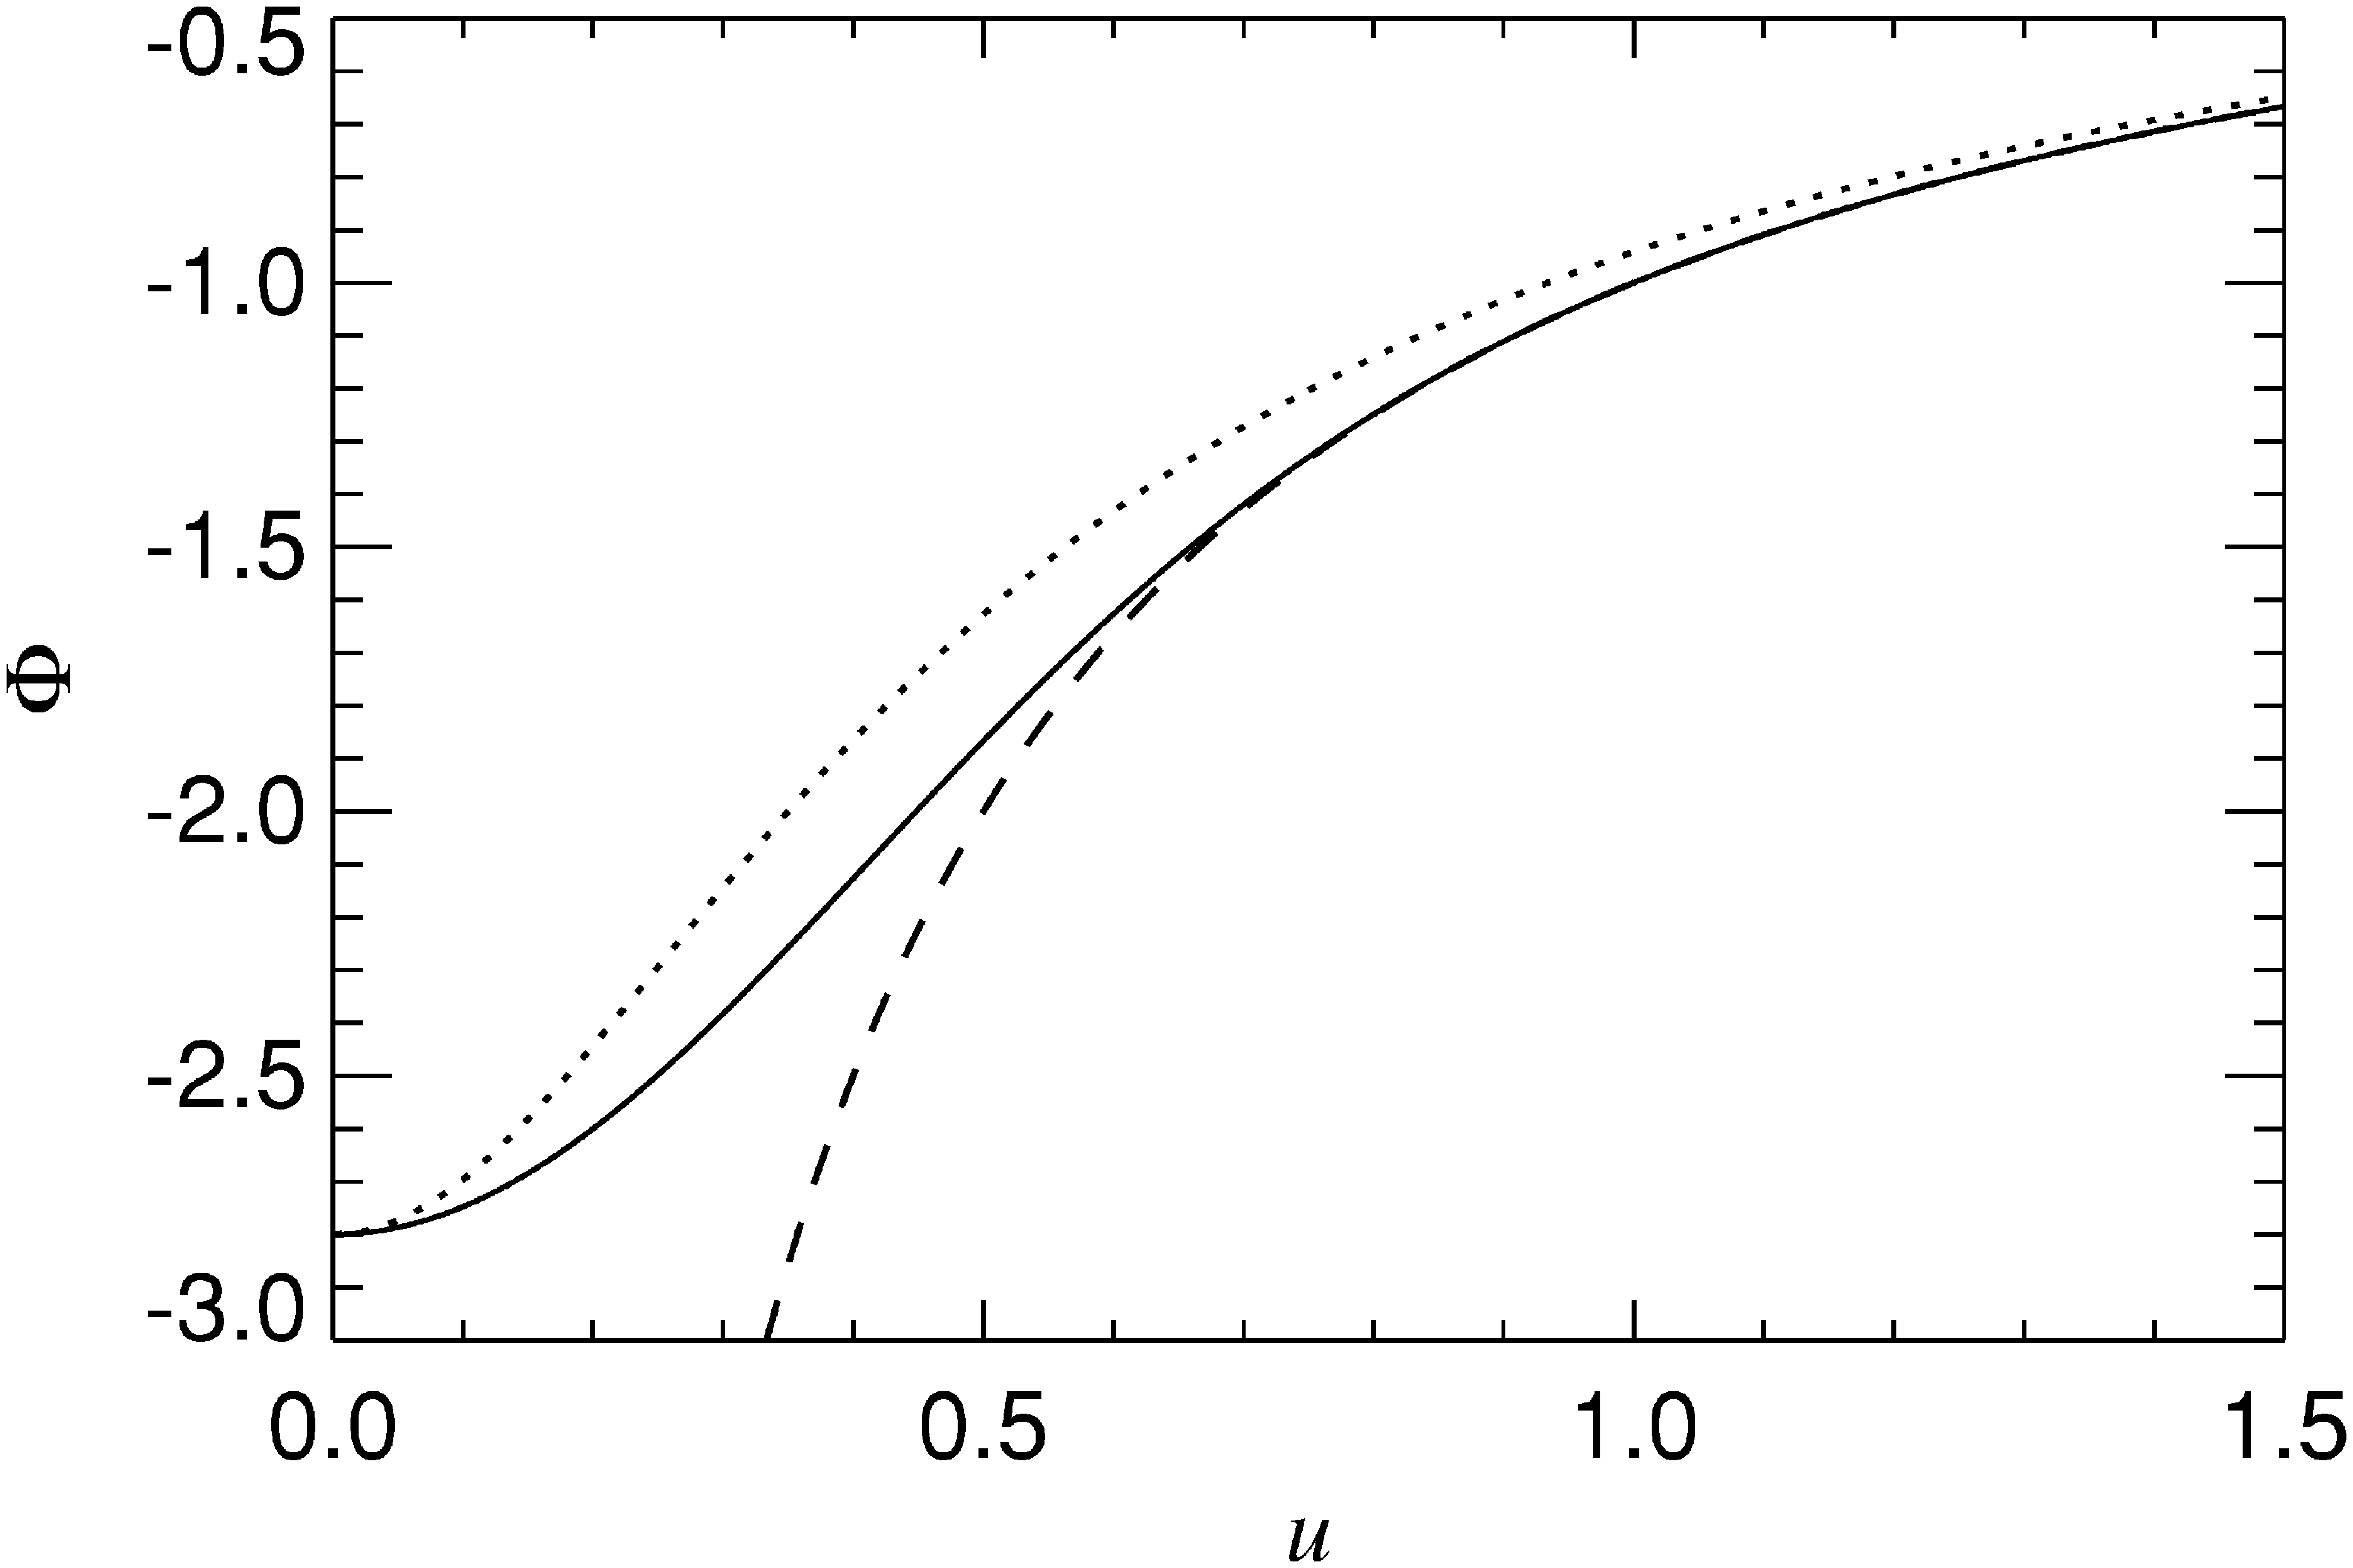
\includegraphics[width=0.48\linewidth]{gadget/softened_potential.eps}
	\end{subfigure}
	\begin{subfigure}{}
		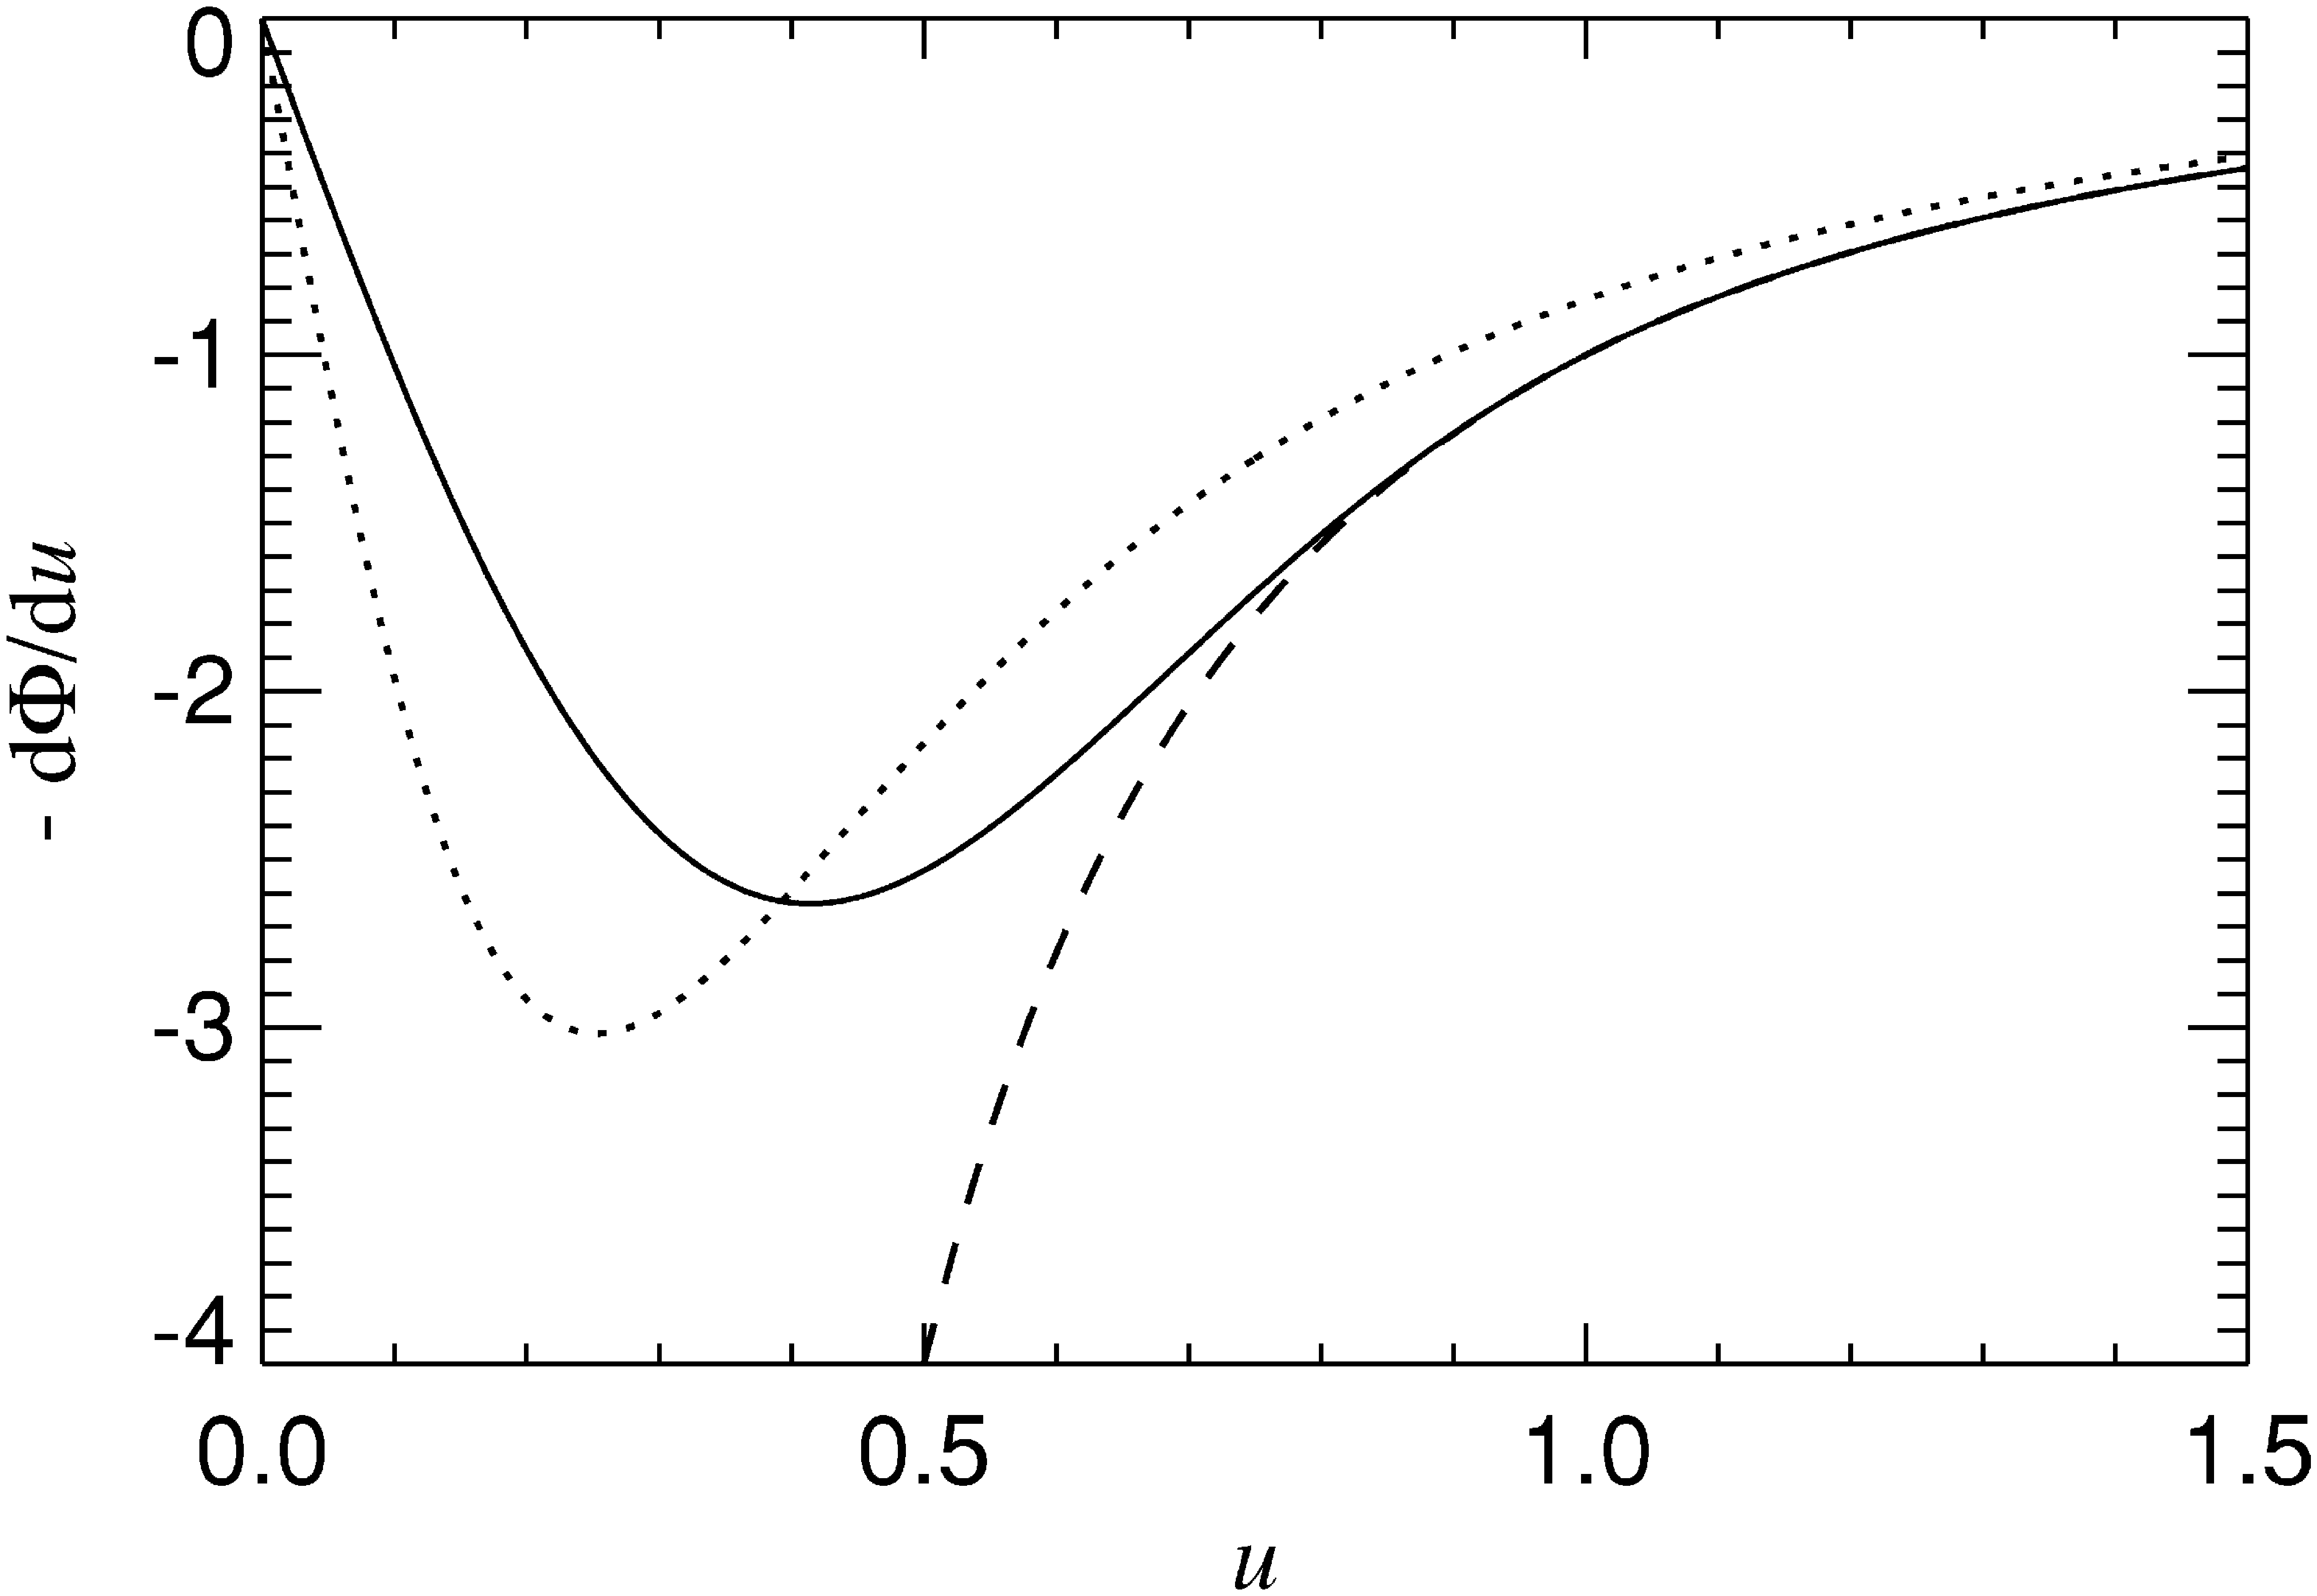
\includegraphics[width=0.48\linewidth]{gadget/softened_force.eps}
	\end{subfigure}
	\caption[Potential and force softening.]{\footnotesize Potential (\emph{left}) and force (\emph{right}) softening.  The solid curves are the spline softening of Equation~\ref{eq:gadget--gadget--spline_kernel}.  Curves for Plummer softening (dotted) and Newton's law (dashed) are provided for comparison.  Here, $h = 1.0$ and $\epsilon = h/2.8$.  \citep{2001NewA....6...79S}}
	\label{fig:gadget--gadget--softening}
\end{figure}

As discussed in Section~\ref{subsec:computational_theory--nbody_simulations}, direct summation \nbody\ techniques are prohibitively slow for modern simulations.  \gadgettwo\ therefore makes use of a hierarchical multipole expansion technique, often called a ``tree'' algorithm, using the Barnes-Hut octal tree \citep{1986Natur.324..446B} algorithm.  This method recursively divides the simulation volume into eight cells at each level of refinement, continuing the division until each cell contains only one particle.  A visual description of this process in two dimensions is given in Figure~\ref{fig:gadget--gadget--tree}.  Distant particles can then be grouped together for the force calculation, reducing the algorithm complexity to $\mathcal{O} (N \log N)$.

\begin{figure}[t]
	\centering
	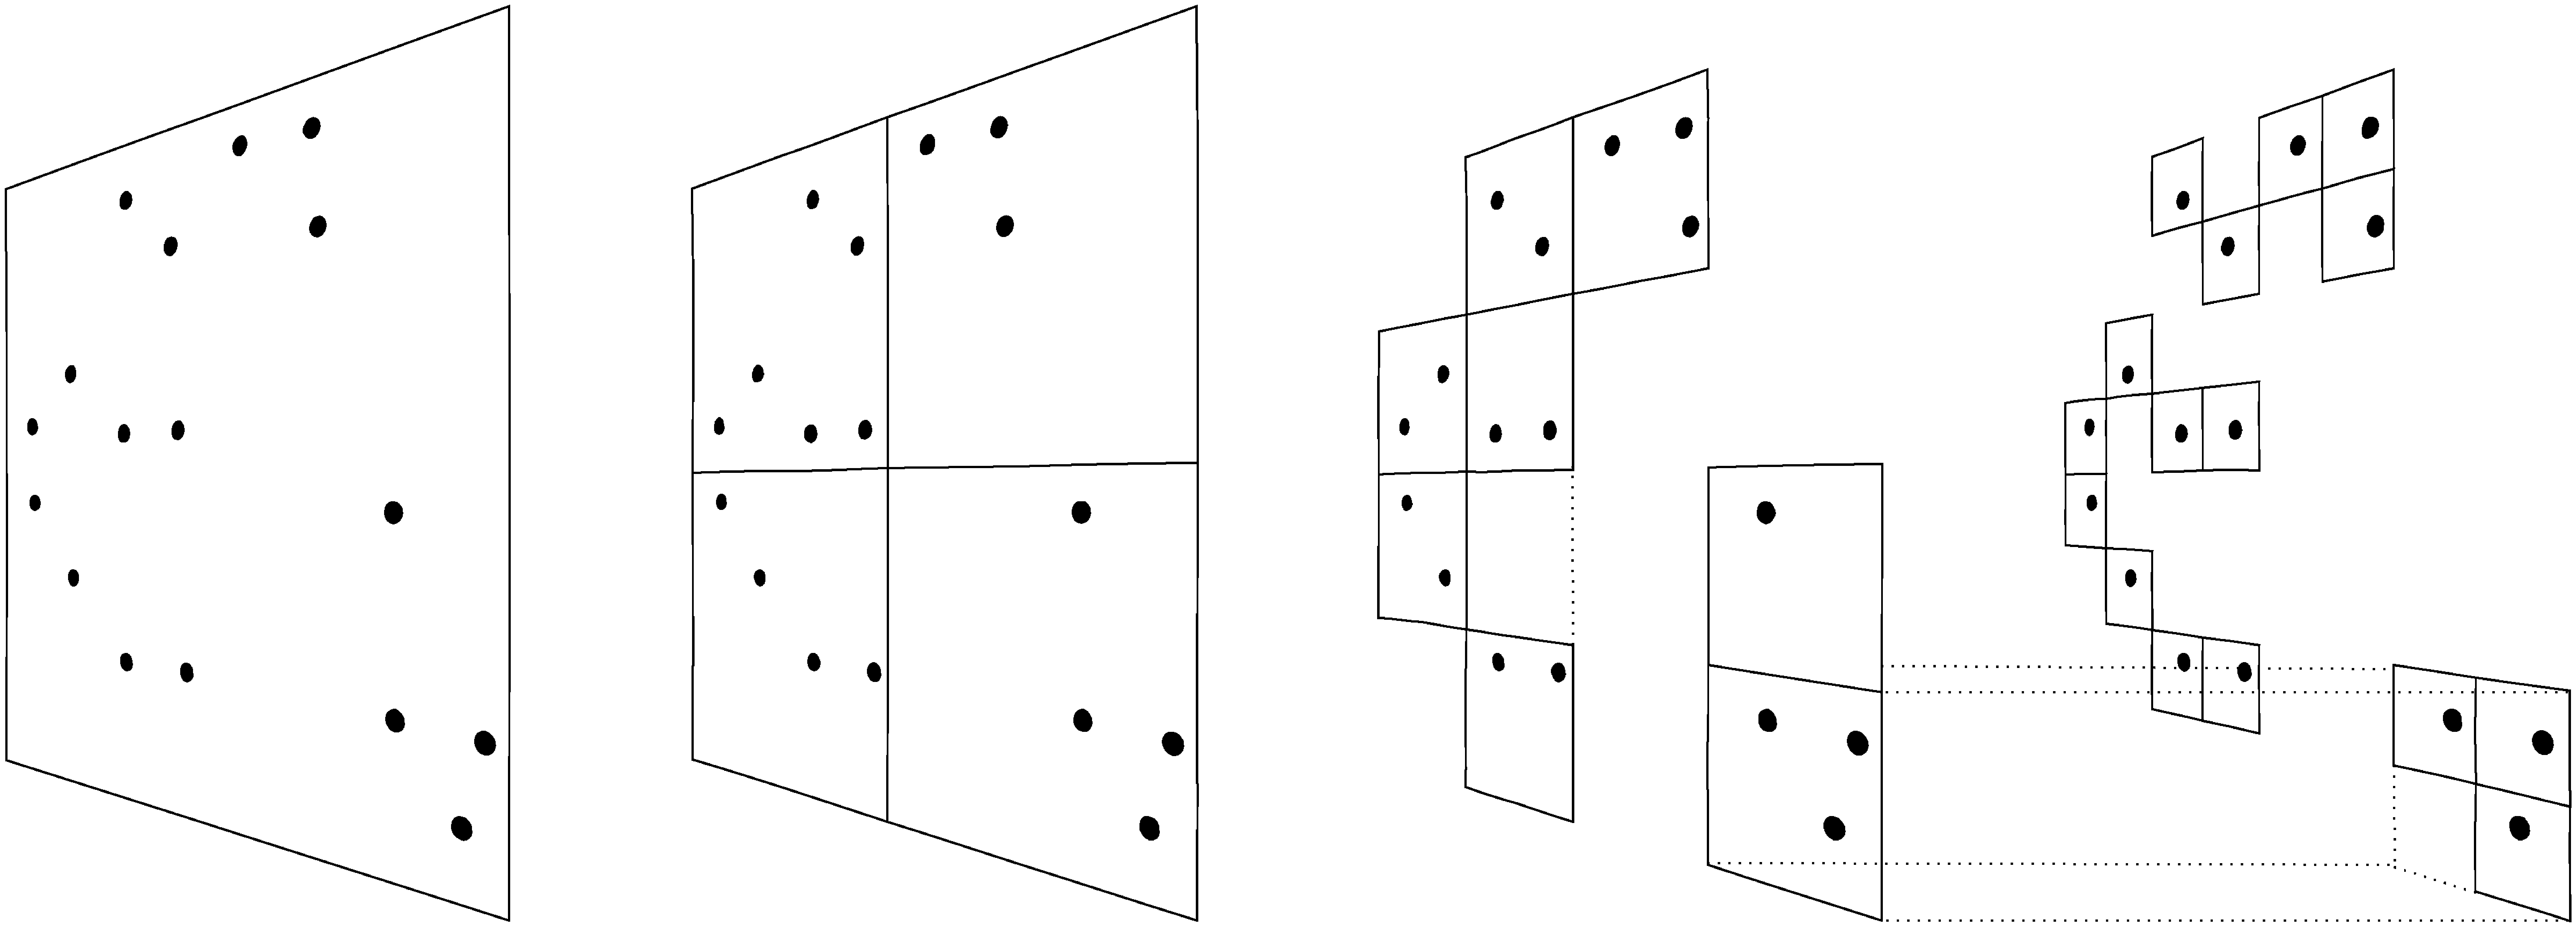
\includegraphics[width=\linewidth]{gadget/tree.eps}
	\caption[Barns-Hut oct-tree in two dimensions.]{\footnotesize Barns-Hut oct-tree in two dimensions.  The simulation volume is recursively partitioned into cells until each contains only one particle each.  Empty cells may be ignored.  \citep{2001NewA....6...79S}}
	\label{fig:gadget--gadget--tree}
\end{figure}

The Barnes-Hut octal tree algorithm begins with a cubic cell encompassing the entire simulation volume.  The cell is then divided into eight daughter cells.  If the cell contains no particles, it is ignored.  If it contains one particle, the dividing process for that cell ends there.  If it contains more than one particle, the process continues recursively, dividing daughter cells into eight octants each, until each cell contains either one or no particles.  A multipole expansion of all daughter cells is then found for each node, or ``leaf.''

The accuracy of the force computation can be set by choosing how far to ``walk'' the tree.  For each particle, the goal is to calculate the gravitational accelerations from all other particles accurately and quickly.  There is a trade off, however, as increasing the accuracy of the tree code toward that of a direct summation approach also increases the runtime complexity toward that of an $\mathcal{O}(N^{2})$ algorithm.  The balance between runtime and accuracy is controlled by the opening angle parameter $\alpha$.  A node of mass $M$ and extension $l$ will be considered for usage if
\begin{equation}
	\frac{GM}{r^{2}} \left( \frac{l}{r} \right)^{2} \leq \alpha |a|,
\end{equation}
where $r$ is the distance from the particle to the node and $|a|$ is the total acceleration from the previous time-step.  Nodes that are massive, large, and near enough to fall outside this criterion are opened so that the daughter cells are recursively considered.

\gadgettwo\ can optionally make use of a hybrid approach for calculating forces, called the TreePM method \citep{1995ApJS...98..355X, 2000ApJS..128..561B, 2002JApA...23..185B}, where long range forces are computed using a particle-mesh algorithm instead of the Barnes-Hut octal tree.  The \gadgettwo\ implementation of TreePM follows that of \citet{2003NewA....8..665B}.



%:::::::::::::::::::::::::::::::::::::::::::::::::::::::::::::::::::::::::::::::
\subsubsection{Time Integration}
\label{subsubsec:gadget--gadget--time_integration}
%:::::::::::::::::::::::::::::::::::::::::::::::::::::::::::::::::::::::::::::::


The \nbody\ Hamiltonian is separable such that $H = H_{\mathrm{kin}} + H_{\mathrm{pot}}$.  Time evolution operators for each of $H_{\mathrm{kin}}$ and $H_{\mathrm{pot}}$ may be computed exactly, leading to ``drift'' and ``kick'' operators \citep{1997astro.ph.10043Q}:
\begin{equation}
	D_{t}(\Delta t):
	\begin{cases}
		p_{i} & \mapsto \; \; \; p_{i}, \\
		x_{i} & \mapsto \; \; \; x_{i} + \displaystyle \frac{p_{i}}{m_{i}} \displaystyle \int_{t}^{t + \Delta t} \frac{\diff t}{a^{2}},
	\end{cases}
\end{equation}
\begin{equation}
	K_{t}(\Delta t):
	\begin{cases}
		x_{i} & \mapsto \; \; \; x_{i}, \\
		p_{i} & \mapsto \; \; \; p_{i} + f_{i} \displaystyle \int_{t}^{t + \Delta t} \frac{\diff t}{a},
	\end{cases}
\end{equation}
where
\begin{equation}
	f_{i} = -\sum_{j} m_{i} m_{j} \frac{\partial \phi(x_{ij})}{\partial x_{i}}
\end{equation}
is the force in particle $i$.

A time evolution operator $U(\Delta t)$ for an interval $\Delta t$  may be approximated by combining the above two operators, where each fall a half time-step after the previous operation:
\begin{equation}
	\tilde{U}(\Delta t) = D \left( \frac{\Delta t}{2} \right) K(\Delta t) D \left( \frac{\Delta t}{2} \right),
\end{equation}
or
\begin{equation}
	\tilde{U}(\Delta t) = K \left( \frac{\Delta t}{2} \right) D(\Delta t) K \left( \frac{\Delta t}{2} \right),
\end{equation}
which gives us a leapfrog integrator constructed as a drift-kick-drift (DKD) or kick-drift-kick (KDK) operator.  DKD and KDK are symplectic and time reversible, as both $D_{i}$ and $K_{i}$ are symplectic.

Cosmological simulations inherently contain a large dynamic range in time scales.  Maintaining a constant time-step would be computationally prohibitive and wasteful, as high-density regions like the centers of galaxies require orders of magnitude smaller time-steps than low-density regions like the intergalactic medium.  \gadgettwo\ therefore uses adaptive individual time-steps which are much more computationally efficient.  The time-step criterion for collisionless particles is
\begin{equation}
	\Delta t_{\mathrm{grav}} = \min \left[ \Delta t_{\max}, \left( \frac{2 \eta \epsilon}{|a|} \right)^{1/2} \right],
\end{equation}
where $\eta$ is an accuracy parameter, $\epsilon$ is the gravitational softening, and $a$ is the particle's acceleration.  The maximum allowed time-step is $\Delta t_{\max}$, which is usually chosen to be a small fraction of the dynamical time of the system.

\gadgettwo\ allows particles to take on time-steps as a power of two subdivision of a global time-step.  A particle is allowed to move to a smaller time-step at any time.  However, moving to a larger time-step is only allowed on every second iteration and when this would lead to synchronization with the higher time-step hierarchy.




%~~~~~~~~~~~~~~~~~~~~~~~~~~~~~~~~~~~~~~~~~~~~~~~~~~~~~~~~~~~~~~~~~~~~~~~~~~~~~~~
\subsection{Simulations}
\label{subsec:gadget--simulations}
%~~~~~~~~~~~~~~~~~~~~~~~~~~~~~~~~~~~~~~~~~~~~~~~~~~~~~~~~~~~~~~~~~~~~~~~~~~~~~~~


We use \gadgettwo\ to evolve six dark matter--only cosmological volumes from $z_{start} = 300$ to $z = 6$ in a $\rm \Lambda CDM$ universe.  Each simulation is initialized using WMAP-5 \citep{2009ApJS..180..330K} parameters.  For each of the three simulation pairs, we directly compare \lpt\ and \za\ by identically sampling the CMB transfer function and displacing the initial particle positions to the same starting redshift using \lpt\ and \za.  The three sets of simulations differ only by the initial phase sampling random seed.  Each volume contains $512^{3}$ particles in a 10 $h^{-1}$ Mpc box.

Following \citet{2010ApJ...715..104H}, we choose conservative simulation parameters in order to ensure high accuracy in integrating the particle positions and velocities.  We have force accuracy of 0.002, integration accuracy of 0.00125, and softening of $0.5\ h^{-1}\ \mathrm{kpc}$, or $1 / 40$ of the initial mean particle separation.  We use a uniform particle mass of $5.3 \times 10^{5} h^{-1} \Msun$.  We select PMGRID, which defines the Fourier grid, to be 1024, SMTH, which defines the split between short- and long-range forces, to be 1.5 times the mesh cell size, and RCUT, which controls the maximum radius for short-range forces, to be 6.0 times the mesh cell size.




